\documentclass{article}

\usepackage{kern}

\begin{document}
    Wir verwenden unter Betrachtung einer Translalation in $C$ Richtung die Fitfunktion
    \[
        f(C + C_0,L) = \frac{1}{\sqrt{L\cdot (C + C_0)}}.
    \]

    \begin{table}[h]
        \centering
        \begin{tabular}{c|ll|ll}
             \textbf{Durchgang} & $L$ in $\si{\henry}$ & $u(L)$ in $\si{\henry}$ & $C$ in $\si{\farad}$ & $u(C)$ in $\si{\farad}$ \\
            \hline
            $1$ & $1.64\cdot 10^{-8}$ & $2.34\cdot 10^{-11}$ & $4.27$ & $0.02$ \\
            $2$ & $1.64\cdot 10^{-8}$ & $2.34\cdot 10^{-11}$ & $4.27$ & $0.02$ \\
        \end{tabular} 
        \caption{Parameterübersicht der Funktion $f(C,L)$ für die aufgenommenen Messwerte.}
    \end{table}


    \begin{figure}[H]
        \centering
        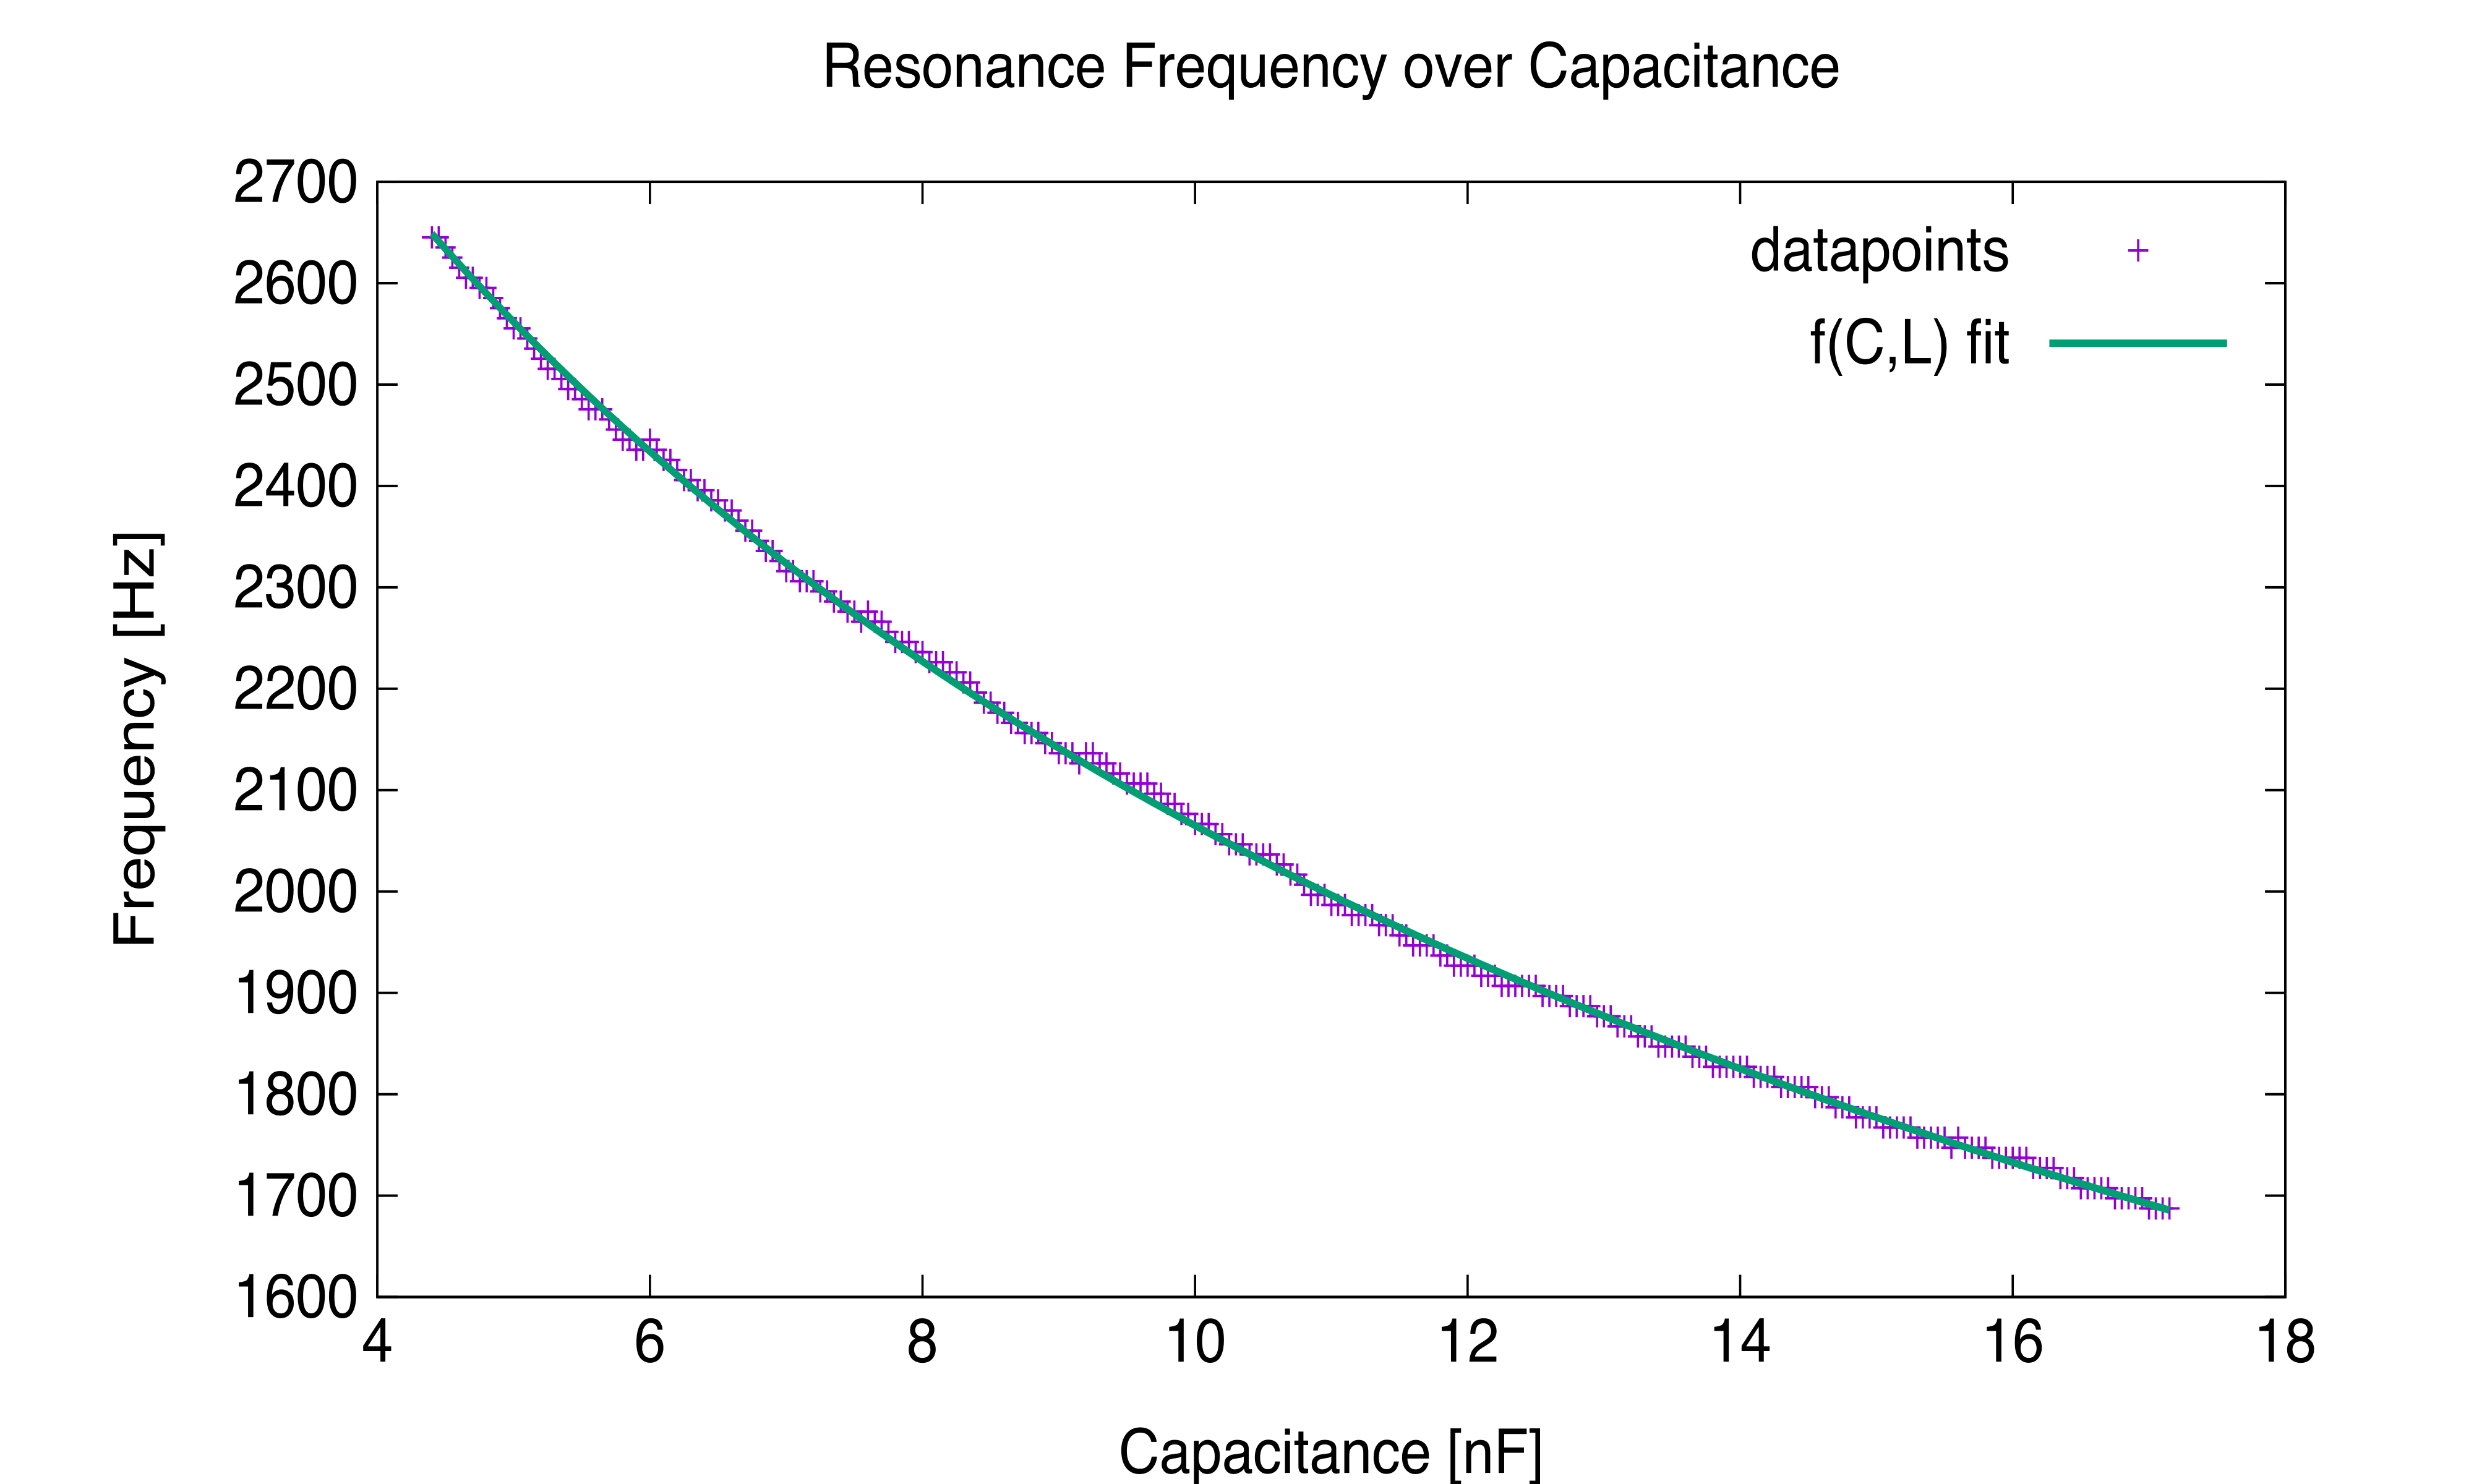
\includegraphics[width=11cm]{../Bilddateien/Messung1_Resonance_Freq_vs_Capacitance.png}
        \caption{Messung der Resonanzfrequenz in Abhängigkeit der Kapazität am Beispiel des ersten Versuchdurchgangs.}
    \end{figure}

\end{document}